\section{Teoría de conjuntos}

\subsection{Introducción}

El concepto de conjunto, es fundamental en matemáticas. Su estudio, se basa en
el hecho de que éstos pueden ser combinados, mediante ciertas operaciones, para
formar otros conjuntos. 

El estudio de las operaciones con los conjuntos, constituye el álgebra de
conjuntos; que tiene semejanzas formales (aunque también presenta diferencias)
con el álgebra de los números. El álgebra de conjuntos, resulta valiosa en la
reducción de los conceptos matemáticos a sus fundamentos lógicos. 

La disciplina matemática que estudia las propiedades generales de los conjuntos
es la teoría de conjuntos. Esta disciplina se comenzó a desarrollar,
rigurosamente, a finales del siglo XIX y principios del XX. El fundador de dicha
teoría es el matemático alemán de origen ruso, George Ferdinand Ludwing
Phillipp Cantor (1845, 1918). Las ideas y conceptos de la teoría de conjuntos
han irrumpido literalmente en todas las ramas de las matemáticas y cambiaron su
faz por completo.

\subsection{Definición básica de conjunto}

Un conjunto es cualquier colección de objetos bien definidos por medio de alguna
o algunas propiedades en común, de dichos objetos. Por objeto entenderemos no
sólo cosas físicas, como discos, computadores, etc., si no también abstractos,
como son números, letras, etc. A los objetos se les llama elementos del
conjunto.

Representamos a los conjuntos por medio de letras mayúsculas, así A, B, C, etc.
nos representan conjuntos.

\subsection{Elemento}

Se llaman elementos o miembros a los objetos que componen un conjunto; y se
denotan con letras minúsculas, como: $a, b, x, y$, etc. Para indicar que un
objeto $x$ pertenece o es miembro de un conjunto $A$, escribimos $x \in A$, que
se lee \textit{“x elemento de A”} y, si no pertenece al conjunto $A$, escribimos
$x \notin A$, que se lee \textit{“x no es elemento de A”}.

\subsection{Conjunto universo}
Llamamos conjunto universo y lo denotamos por U, al conjunto del cual se
seleccionan los elementos para formar conjuntos.

En general identificamos al conjunto universo como un todo, pero no
representamos de una manera única a este “todo”, así habrá ocasiones que un
conjunto sea considerado conjunto universo y en otras no, por ejemplo:
considerando el conjunto P de los número pares, se tiene que $\mathbb Z$
(conjunto enteros) es un conjunto universo para él; pero si consideramos el
mismo conjunto $\mathbb Z$, tenemos que $\mathbb Q$ (racionales) es un conjunto
universo de él. Así Z es un conjunto universo en ocasiones y en otras no. Además
puede haber varios conjuntos universos para un solo conjunto, por ejemplo el
mismo conjunto P de números pares tiene por conjunto universo a $\mathbb Z$
(conjunto de los enteros) o a Q (conjunto se los racionales) o a $\mathbb R$
(conjunto de los reales) o incluso a $\mathbb C$ (conjunto de los complejos), en
general podemos decir que para números el conjunto universo más grande es
$\mathbb C$ (números complejos).

\subsection{Conjunto vacío}

El conjunto vacío o nulo es un conjunto que no tiene elementos, el conjunto
vacío se representa por: $\emptyset$, o bien por {}.

No confundir el conjunto $A = \emptyset $ con el conjunto $ A = {\emptyset} $,
ya que el primer conjunto indica que no tiene ningún elemento y el segundo
conjunto indica que tiene un elemento y ese elemento es el conjunto vacío.

\subsection{Igualdad de conjuntos}

Decimos que dos conjuntos $A$ y $B$ son iguales y denotamos $A=B$, si $A$ y $B$
constan de los mismos elementos, i.e. si cada elemento de $A$ pertenece a $B$ y
si cada elemento de $B$ pertenece a $A$.

\subsection{Subconjunto}

Si todos los elementos de un conjunto A son también elementos de un conjunto
$B$, esto es, si cuando $x \in A$ entonces $x \in B$ (simbólicamente $x \in A
\rightarrow x \in B$), decimos que A es un subconjunto de B o que A está
contenido en B y se escribe:

\begin{equation}
    \begin{array}{l}
        A \subseteq B \\
        B \subseteq A
    \end{array}
\end{equation}

Si $A$ no es subconjunto de $B$ se escribe $A \not \subset B$ .

Si además existe un elemento de $B$ que no este en $A$, decimos que $A$ es un
subconjunto propio de $B$ y se denota $A \subset B$ o $B \subset A$.

\subsection{Propiedades de los conjuntos}

\begin{enumerate}
    \item Si A es cualquier conjunto diferente del vacío, entonces $A \subseteq A$ . Esto es, cualquier conjunto
    diferente del vacío es subconjunto de si mismo.
    
\item El conjunto vacío es subconjunto de cualquier conjunto distinto del vacío,
esto es $\emptyset \subset A$

\item Si $n>0$ es el número de elementos de $A$ entonces el número de elementos de $P(A)$ es $2^n$
\end{enumerate}

\begin{theorem}{Conjuntos}{conjuntos}
Sean $A$ y $B$ dos conjuntos. Decimos que $A=B$ si y solo si $A \subseteq B$ y
$B \subseteq A$
\end{theorem}

\begin{theorem}{Conjuntos}{conjuntos}
    Si $ A \subset B $ y $ B \subset C $, entonces $ A \subset C $
\end{theorem}

\subsection{Cardinalidad}

Sea $A$ un conjunto, la cardinalidad de $A$ es el número de elementos diferentes del conjunto
$A$ y se representa por $|A|$.

\subsection{Conjunto potencia}
Sea $A$ un conjunto finito, llamaremos conjunto potencia al conjunto formado por todos los
subconjuntos de $A$. El conjunto potencia se denota como $P(A)$ o bien $2^A$.

\subsection{Operaciones entre conjuntos}

% Definition of circles
\def\firstcircle{(0,0) circle (1.5cm)}
\def\secondcircle{(0:2cm) circle (1.5cm)}

\colorlet{circle edge}{blue!50}
\colorlet{circle area}{blue!20}

\tikzset{filled/.style={fill=circle area, draw=circle edge, thick},
    outline/.style={draw=circle edge, thick}}

\setlength{\parskip}{5mm}

\subsubsection{Unión}

La unión La unión (o reunión) de dos conjuntos $A$ y $B$, denotada por $ A \cup
B $ (que se lee “A unión B”) es un nuevo conjunto formado por los elementos que
pertenecen a A o a B o a ambos conjuntos.

\begin{equation}
    A \cup B = {x | x \in A \vee x \in B}
\end{equation}

Si $x \in A \cup B $ entonces $x \in A $ ó $x \in B$ o $x$ pertenece a ambos
conjuntos.

% Set A or B
\begin{figure}[h]
    \centering
    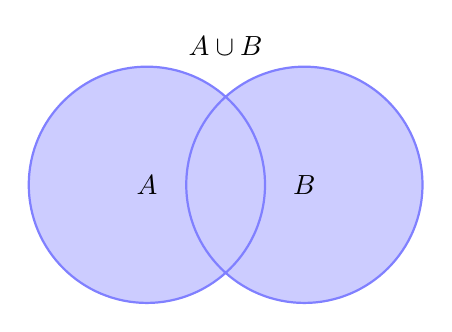
\begin{tikzpicture}
        \draw[filled] \firstcircle node {$A$}
                      \secondcircle node {$B$};
        \node[anchor=south] at (current bounding box.north) {$A \cup B$};
    \end{tikzpicture}
\end{figure}

\subsubsection{Intersección}

La intersección de dos conjuntos $A$ y $B$, denotada por $A \cap B$ (que se lee “ A intersección B”),
es un nuevo conjunto formado por los elementos que pertenecen a A y a B al mismo tiempo, es
decir, por los elementos comunes a ambos conjuntos.

\begin{equation}
    A \cap B={x | x \in A \wedge x \in B}
\end{equation}

% Set A and B
\begin{figure}[h]
    \centering
    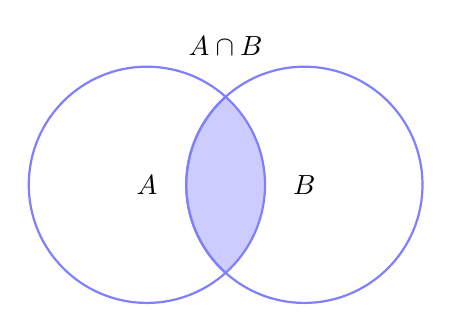
\begin{tikzpicture}
        \begin{scope}
            \clip \firstcircle;
            \fill[filled] \secondcircle;
        \end{scope}
        \draw[outline] \firstcircle node {$A$};
        \draw[outline] \secondcircle node {$B$};
        \node[anchor=south] at (current bounding box.north) {$A \cap B$};
    \end{tikzpicture}
\end{figure}

\subsubsection{Complemento}

Sea $A \subseteq U$ un conjunto. El complemento de A denotado por $A'$, $A^C$ ó $U-A$, se define
como el conjunto de todos los elementos que están en $U$ pero no están en $A$.
Simbólicamente:

\begin{equation}
    \bar{A}= {x | x \in U \wedge x \notin A}
\end{equation}

Es decir, el complemento de $A$ es el conjunto de los todos los elementos que no
están en el conjunto $A$. Simbólicamente: $ \bar{A}={x | x \notin A}$.

\subsubsection{Diferencia}

% Set A but not B
\begin{figure}[h]
    \centering
    \begin{subfigure}[b]{0.45\textwidth}
        \centering
        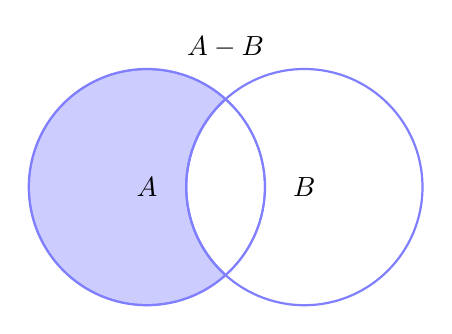
\begin{tikzpicture}
            \begin{scope}
                \clip \firstcircle;
                \draw[filled, even odd rule] \firstcircle node {$A$}
                                             \secondcircle;
            \end{scope}
            \draw[outline] \firstcircle
                           \secondcircle node {$B$};
            \node[anchor=south] at (current bounding box.north) {$A - B$};
        \end{tikzpicture}
    \end{subfigure}
\hfill
    \begin{subfigure}[b]{0.45\textwidth}
        \centering
        % Set B but not A
        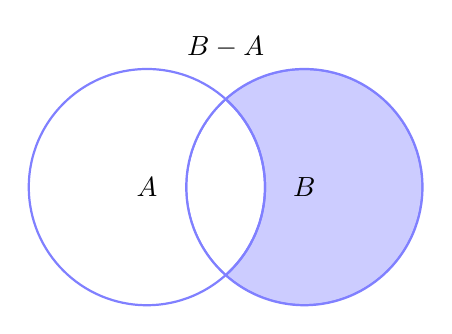
\begin{tikzpicture}
            \begin{scope}
                \clip \secondcircle;
                \draw[filled, even odd rule] \firstcircle
                                             \secondcircle node {$B$};
            \end{scope}
            \draw[outline] \firstcircle node {$A$}
                           \secondcircle;
            \node[anchor=south] at (current bounding box.north) {$B - A$};
        \end{tikzpicture}
\end{subfigure}
\end{figure}

\subsubsection{Diferencia simétrica}



%Set A or B but not (A and B) also known a A xor B
\begin{figure}[h]
    \centering
    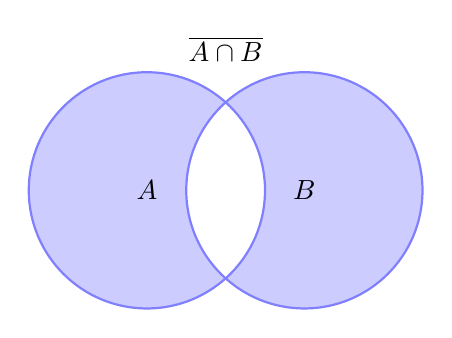
\begin{tikzpicture}
        \draw[filled, even odd rule] \firstcircle node {$A$}
                                     \secondcircle node{$B$};
        \node[anchor=south] at (current bounding box.north) {$\overline{A \cap B}$};
    \end{tikzpicture}
\end{figure}



